\documentclass[a4paper,11pt]{article}
\usepackage[utf8]{inputenc}
\usepackage[T1]{fontenc}
\usepackage{amsmath,amssymb}
\usepackage[a4paper,left=2cm,right=2cm,top=3.6cm,bottom=2.3cm,headheight=1.1cm,headsep=0.6cm,footskip=1cm]{geometry}
\usepackage{xcolor}
\usepackage{tikz}
\usetikzlibrary{calc,arrows.meta,positioning,shapes.geometric}
\usepackage{fancyhdr}
\usepackage{lastpage}
\usepackage{tabularx}
\usepackage{array}
\usepackage[most]{tcolorbox}
\usepackage{enumitem}
\usepackage{needspace}

% ---------- palet teal ----------
\definecolor{tealx}{HTML}{0F766E}
\definecolor{aquax}{HTML}{14A89A}
\definecolor{deepx}{HTML}{134E4A}
\definecolor{softbg}{HTML}{E8F6F4}
\definecolor{coralx}{HTML}{E4673F}
\newcommand{\dis}{\displaystyle}

\setlength{\parindent}{0pt}
\renewcommand{\arraystretch}{1.35}

\tikzset{
  ar/.style={-{Stealth[length=1.8mm]},thick,tealx},
  box/.style={draw=tealx,thick,rounded corners=3pt,fill=softbg,align=center,inner sep=4pt},
  gr/.style={gray!30,very thin},
  ax/.style={-{Stealth[length=1.6mm]},thick,deepx},
  orig/.style={thick,deepx,dashed},
  img/.style={very thick,coralx},
  cur/.style={very thick,tealx}
}

% ---------- header berwarna teal ----------
\pagestyle{fancy}
\fancyhf{}
\renewcommand{\headrulewidth}{0pt}
\fancyhead[L]{%
  \begin{tikzpicture}[remember picture,overlay]
    \fill[tealx] ([yshift=-1.2cm]current page.north west) rectangle ([yshift=-3.15cm]current page.north east);
    \fill[aquax] ([yshift=-3.15cm]current page.north west) rectangle ([yshift=-3.25cm]current page.north east);
  \end{tikzpicture}%
  \color{white}\bfseries\large Latihan Soal Transformasi Fungsi}
\fancyhead[R]{\color{white}\small Diunduh dari website \textbf{Math1729}\ \,|\,\ 4 Oktober 2026}
\fancyfoot[L]{\small\color{tealx}Math1729 --- Transformasi Fungsi}
\fancyfoot[R]{\small\color{tealx}Halaman \thepage\ dari \pageref{LastPage}}

% ---------- komponen ----------
\newcounter{no}
\newcommand{\bagian}[2]{\par\Needspace{6\baselineskip}\vspace{1.0em}\noindent
  \begin{tcolorbox}[colback=tealx,colframe=tealx,coltext=white,boxrule=0pt,arc=2pt,left=6pt,right=6pt,top=3pt,bottom=3pt]
  \textbf{#1}\hfill{\small #2}\end{tcolorbox}\setcounter{no}{0}\par\vspace{-0.3em}}
\newcommand{\tingkat}[2]{\par\Needspace{7\baselineskip}\vspace{0.6em}\noindent
  {\color{aquax}\rule{3pt}{1.1em}}\ {\color{tealx}\bfseries #1}\ {\small\color{gray}--- #2}\par\vspace{0.1em}}
\newcommand{\soal}[2]{\par\vspace{0.75em}\stepcounter{no}\noindent
  \begin{minipage}[t]{1.8em}\textbf{\theno.}\end{minipage}%
  \begin{minipage}[t]{\dimexpr\linewidth-1.8em\relax}#1\par\vspace{0.35em}#2\end{minipage}\par}
\newcommand{\poin}[1]{\hfill{\small\color{tealx}[#1 poin]}}

% teks di kiri, gambar di kanan
\newcommand{\gbr}[2]{\noindent\begin{minipage}[t]{0.52\linewidth}#1\end{minipage}\hfill\raisebox{\ht\strutbox}{\begin{minipage}[t]{0.45\linewidth}\vspace{0pt}\centering#2\end{minipage}}}

% pilihan jawaban
\newcommand{\pil}[5]{\begin{tabularx}{\linewidth}{@{}*{5}{X}@{}}\textbf{A.}\;#1 & \textbf{B.}\;#2 & \textbf{C.}\;#3 & \textbf{D.}\;#4 & \textbf{E.}\;#5\end{tabularx}}
\newcommand{\pilx}[5]{\begin{tabularx}{\linewidth}{@{}*{3}{>{\raggedright\arraybackslash}X}@{}}\textbf{A.}\;#1 & \textbf{B.}\;#2 & \textbf{C.}\;#3\\[10pt] \textbf{D.}\;#4 & \textbf{E.}\;#5 & \end{tabularx}}
\newcommand{\jwb}{\hfill Jawaban: \rule{4.5cm}{0.4pt}}

\begin{document}
\thispagestyle{fancy}

\begin{center}
  {\color{tealx}\fontsize{22}{26}\selectfont\bfseries Latihan Soal Transformasi Fungsi\par}
  \vspace{2pt}
  {\color{aquax}\large Translasi, Refleksi, Dilatasi, Rotasi, Nilai Mutlak, Komposisi, dan Transformasi Matriks\par}
\end{center}
\vspace{2pt}
\begin{tcolorbox}[colback=softbg,colframe=tealx!40,boxrule=0.6pt,arc=3pt,left=8pt,right=8pt,top=5pt,bottom=5pt]
\noindent\textbf{Nama} : \rule{4.6cm}{0.4pt}\hfill\textbf{Kelas} : \rule{2.2cm}{0.4pt}\hfill\textbf{Skor} : \rule{2.2cm}{0.4pt}
\end{tcolorbox}
\vspace{2pt}
\begin{tcolorbox}[colback=white,colframe=aquax,boxrule=0.8pt,arc=3pt,left=8pt,right=8pt,top=4pt,bottom=4pt,title={\bfseries Petunjuk Pengerjaan},coltitle=white,fonttitle=\small]
\small
\begin{enumerate}[leftmargin=1.4em,itemsep=1pt,topsep=1pt]
\item Soal terdiri atas \textbf{20 pilihan ganda} (5 mudah, 5 sedang, 5 sulit, 5 HOTS), \textbf{5 isian singkat}, dan \textbf{5 uraian (essay)}. Bentuk soal mengikuti pola UTBK-SNBT terbaru: pilihan ganda lima opsi, \textbf{pilihan majemuk kompleks} (tabel Benar/Salah, soal PG nomor 18), isian singkat, soal berbasis konteks dan grafik, analisis kesalahan pengerjaan, serta kecukupan data. Alokasi waktu yang disarankan: 120 menit.
\item Skor: pilihan ganda 2 poin, isian singkat 4 poin, uraian 8 poin per soal (total 100 poin). Soal pilihan majemuk kompleks bernilai penuh hanya jika keempat pernyataan dijawab benar. Tidak ada pengurangan skor untuk jawaban salah.
\item Kesepakatan: translasi $T=(h,k)$ memetakan $(x,y)$ ke $(x+h,y+k)$. Rotasi bernilai positif jika berlawanan arah jarum jam. Dilatasi $[P,k]$ berpusat di $P$ dengan faktor skala $k$. Gambar tidak selalu digambar sesuai skala.
\item Bilangan desimal ditulis dengan tanda koma. Kalkulator tidak diperkenankan.
\end{enumerate}
\end{tcolorbox}

% =====================================================================
\bagian{A. Pilihan Ganda}{20 soal $\times$ 2 poin = 40 poin. Pilih satu jawaban yang paling tepat.}

\tingkat{Tingkat Mudah}{soal 1 sampai 5}
\soal{\gbr{Gambar di samping menunjukkan grafik $y=f(x)$. Grafik $y=g(x)$ dengan $g(x)=f(x+3)-1$ adalah bayangan grafik $f$. Titik minimum grafik $g$ adalah \dots.}{%
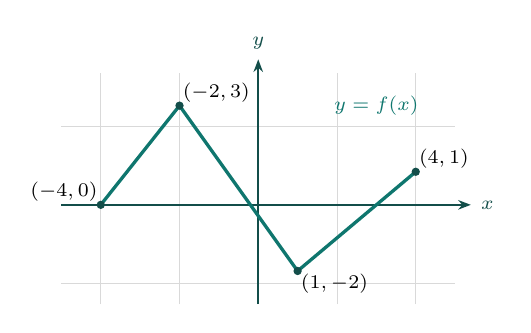
\begin{tikzpicture}[x=0.5cm,y=0.42cm]
\draw[gr] (-5,-3) grid (5,4);
\draw[ax] (-5,0)--(5.4,0) node[right,font=\scriptsize]{$x$};
\draw[ax] (0,-3)--(0,4.4) node[above,font=\scriptsize]{$y$};
\draw[cur] (-4,0)--(-2,3)--(1,-2)--(4,1);
\fill[deepx] (-4,0) circle (1.5pt) (-2,3) circle (1.5pt) (1,-2) circle (1.5pt) (4,1) circle (1.5pt);
\node[font=\scriptsize,above right,inner sep=1pt] at (-2,3) {$(-2,3)$};
\node[font=\scriptsize,below right,inner sep=1pt] at (1,-2) {$(1,-2)$};
\node[font=\scriptsize,above left,inner sep=1pt] at (-4,0) {$(-4,0)$};
\node[font=\scriptsize,above right,inner sep=1pt] at (4,1) {$(4,1)$};
\node[font=\scriptsize,tealx] at (3,3) {$y=f(x)$};
\end{tikzpicture}}}{\pil{$(4,-3)$}{$(-2,-3)$}{$(-2,-1)$}{$(4,-1)$}{$(1,-3)$}}
\soal{Bayangan garis $2x-y+4=0$ oleh pencerminan terhadap garis $x=1$ adalah \dots.}{\pil{$2x+y-4=0$}{$2x+y-6=0$}{$2x+y-8=0$}{$2x+y+2=0$}{$2x-y+8=0$}}
\soal{Grafik $y=f(x)$ mencapai nilai maksimum $6$ di titik $(2,6)$. Titik maksimum grafik $y=\dfrac12f(3x)$ adalah \dots.}{\pil{$(6,3)$}{$(6,12)$}{$\left(\frac23,12\right)$}{$(2,3)$}{$\left(\frac23,3\right)$}}
\soal{Garis $y=2x+1$ diputar sejauh $90^\circ$ berlawanan arah jarum jam dengan pusat $O(0,0)$. Persamaan garis bayangannya adalah \dots.}{\pilx{$y=-\frac12x-\frac12$}{$y=-\frac12x+\frac12$}{$y=\frac12x-\frac12$}{$y=-2x-1$}{$y=\frac12x+\frac12$}}
\soal{\gbr{Gambar menunjukkan grafik $y=|x^2-2x-3|$ (garis tebal) dan grafik $y=x^2-2x-3$ (garis putus-putus). Koordinat titik puncak (maksimum lokal) pada grafik $y=|x^2-2x-3|$ adalah \dots.}{%
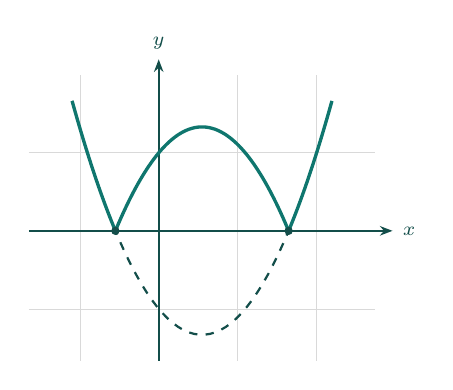
\begin{tikzpicture}[x=0.55cm,y=0.33cm]
\draw[gr] (-3,-5) grid (5,6);
\draw[ax] (-3,0)--(5.4,0) node[right,font=\scriptsize]{$x$};
\draw[ax] (0,-5)--(0,6.6) node[above,font=\scriptsize]{$y$};
\draw[orig,domain=-2:4,samples=50] plot (\x,{\x*\x-2*\x-3});
\draw[cur,domain=-2:-1,samples=20] plot (\x,{\x*\x-2*\x-3});
\draw[cur,domain=-1:3,samples=60] plot (\x,{-(\x*\x-2*\x-3)});
\draw[cur,domain=3:4,samples=20] plot (\x,{\x*\x-2*\x-3});
\fill[deepx] (-1,0) circle (1.5pt) (3,0) circle (1.5pt);
\end{tikzpicture}}}{\pil{$(1,-4)$}{$(-1,0)$}{$(3,0)$}{$(1,4)$}{$(0,3)$}}

\tingkat{Tingkat Sedang}{soal 6 sampai 10}
\soal{Parabola $y=x^2-6x+7$ dicerminkan terhadap garis $y=1$, kemudian hasilnya ditranslasikan oleh $(-2,3)$. Persamaan parabola akhir adalah \dots.}{\pilx{$y=-x^2+2x$}{$y=-x^2+2x+6$}{$y=-x^2+2x+4$}{$y=-x^2+10x-24$}{$y=-x^2+6x-5$}}
\soal{Transformasi $T_1$ adalah pencerminan terhadap garis $y=-x$, dilanjutkan $T_2$ berupa rotasi $90^\circ$ berlawanan arah jarum jam dengan pusat $O$. Titik $(a,b)$ dipetakan oleh $T_1$ yang dilanjutkan $T_2$ menjadi $(-3,5)$. Nilai $a+b$ adalah \dots.}{\pil{$-8$}{$-2$}{$2$}{$8$}{$0$}}
\soal{\gbr{Gambar menunjukkan grafik $y=|x^2-4x+3|$ dan garis mendatar $y=m$ yang dapat digeser naik turun. Jika garis tersebut memotong grafik di tepat tiga titik, nilai $m$ adalah \dots.}{%
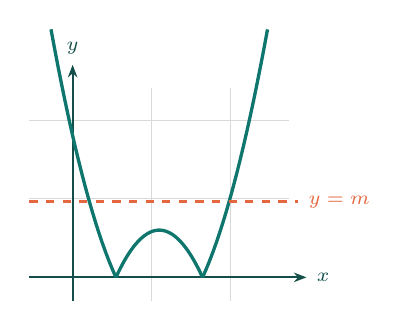
\begin{tikzpicture}[x=0.55cm,y=0.6cm]
\draw[gr] (-1,-0.5) grid (5,4);
\draw[ax] (-1,0)--(5.4,0) node[right,font=\scriptsize]{$x$};
\draw[ax] (0,-0.5)--(0,4.5) node[above,font=\scriptsize]{$y$};
\draw[cur,domain=-0.5:1,samples=20] plot (\x,{\x*\x-4*\x+3});
\draw[cur,domain=1:3,samples=40] plot (\x,{-(\x*\x-4*\x+3)});
\draw[cur,domain=3:4.5,samples=20] plot (\x,{\x*\x-4*\x+3});
\draw[img,dashed] (-1,1.6)--(5.2,1.6) node[right,font=\scriptsize,coralx]{$y=m$};
\end{tikzpicture}}}{\pil{$0$}{$\frac12$}{$1$}{$2$}{$3$}}
\soal{Parabola $y=x^2$ didilatasikan dengan pusat $P(1,2)$ dan faktor skala $2$. Persamaan bayangannya adalah \dots.}{\pilx{$y=2x^2-2x+\frac32$}{$y=\frac12x^2$}{$y=\frac12x^2-x-\frac32$}{$y=x^2+2x-3$}{$y=\frac12x^2+x-\frac32$}}
\soal{\gbr{Grafik $y=g(x)$ pada gambar adalah bayangan grafik $y=f(x)$ oleh transformasi $g(x)=2f(x+1)-3$. Nilai $f(0)+f(2)+f(4)$ adalah \dots.}{%
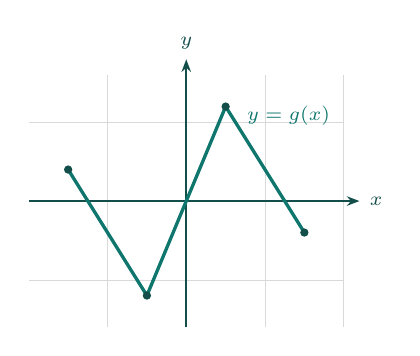
\begin{tikzpicture}[x=0.5cm,y=0.4cm]
\draw[gr] (-4,-4) grid (4,4);
\draw[ax] (-4,0)--(4.4,0) node[right,font=\scriptsize]{$x$};
\draw[ax] (0,-4)--(0,4.5) node[above,font=\scriptsize]{$y$};
\draw[cur] (-3,1)--(-1,-3)--(1,3)--(3,-1);
\fill[deepx] (-3,1) circle (1.5pt) (-1,-3) circle (1.5pt) (1,3) circle (1.5pt) (3,-1) circle (1.5pt);
\node[font=\scriptsize,tealx] at (2.6,2.7) {$y=g(x)$};
\end{tikzpicture}}}{\pil{$-5$}{$-1$}{$8$}{$4$}{$12$}}

\tingkat{Tingkat Sulit}{soal 11 sampai 15, setara UTBK}
\soal{Grafik fungsi $f$ memiliki titik minimum global di $(-1,5)$. Grafik $g(x)=-2f(3-x)+4$ memiliki \dots.}{\pilx{maksimum global di $(-2,-6)$}{minimum global di $(4,-6)$}{maksimum global di $(4,-6)$}{minimum global di $(-2,-6)$}{maksimum global di $(4,-14)$}}
\soal{Grafik $y=\log_2x$ diputar $90^\circ$ berlawanan arah jarum jam dengan pusat $O(0,0)$, kemudian ditranslasikan oleh $(1,-3)$. Absis titik potong grafik akhir dengan sumbu-$x$ adalah \dots.}{\pil{$\log_23-1$}{$1-\log_23$}{$1+\log_23$}{$\log_23$}{$-\log_23$}}
\soal{\gbr{Parabola $y=x^2$ (putus-putus) diputar $180^\circ$ dengan pusat $C(3,10)$ sehingga menghasilkan parabola baru (garis tebal). Kedua parabola berpotongan di dua titik. Jarak antara kedua titik potong tersebut adalah \dots.}{%
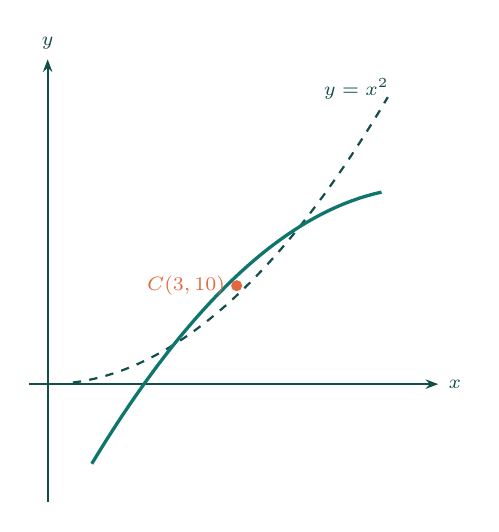
\begin{tikzpicture}[x=0.8cm,y=0.125cm]
\draw[ax] (-0.3,0)--(6.2,0) node[right,font=\scriptsize]{$x$};
\draw[ax] (0,-12)--(0,33) node[above,font=\scriptsize]{$y$};
\draw[orig,domain=0.4:5.4,samples=40] plot (\x,{\x*\x});
\draw[cur,domain=0.7:5.3,samples=40] plot (\x,{-\x*\x+12*\x-16});
\fill[coralx] (3,10) circle (2pt) node[left,font=\scriptsize,inner sep=4pt]{$C(3,10)$};
\node[font=\scriptsize,deepx] at (4.9,30) {$y=x^2$};
\end{tikzpicture}}}{\pil{$2\sqrt{37}$}{$12$}{$4\sqrt{10}$}{$6\sqrt5$}{$2\sqrt{35}$}}
\soal{\gbr{Kurva $A$ adalah bayangan $y=|x|$ oleh translasi $(0,-2)$. Kurva $B$ adalah bayangan $y=|x|$ oleh pencerminan terhadap sumbu-$x$, dilanjutkan peregangan vertikal dengan faktor $2$, lalu translasi $(0,4)$. Luas daerah tertutup yang dibatasi kurva $A$ dan $B$ (daerah arsiran) adalah \dots.}{%
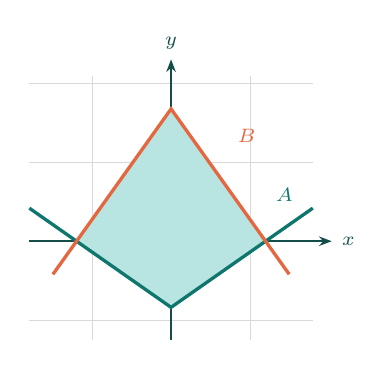
\begin{tikzpicture}[x=0.6cm,y=0.42cm]
\draw[gr] (-3,-3) grid (3,5);
\draw[ax] (-3,0)--(3.4,0) node[right,font=\scriptsize]{$x$};
\draw[ax] (0,-3)--(0,5.5) node[above,font=\scriptsize]{$y$};
\fill[aquax!30] (0,-2)--(2,0)--(0,4)--(-2,0)--cycle;
\draw[cur] (-3,1)--(0,-2)--(3,1);
\draw[img] (-2.5,-1)--(0,4)--(2.5,-1);
\node[font=\scriptsize,tealx] at (2.4,1.4) {$A$};
\node[font=\scriptsize,coralx] at (1.6,3.2) {$B$};
\end{tikzpicture}}}{\pil{$8$}{$9$}{$15$}{$18$}{$12$}}
\soal{Parabola $y=x^2-2x$ ditranslasikan oleh $(1,-2)$, kemudian hasilnya dicerminkan terhadap sumbu-$x$ sehingga diperoleh parabola $P$. Garis $y=3x+k$ menyinggung parabola $P$. Nilai $k$ adalah \dots.}{\pil{$-\frac54$}{$-1$}{$-\frac12$}{$-\frac34$}{$\frac34$}}

\Needspace{20\baselineskip}\tingkat{Tingkat HOTS}{soal 16 sampai 20, penalaran tingkat tinggi gaya UTBK}
\soal{Rani diminta menentukan bayangan kurva $y=x^2-2x$ oleh dilatasi pusat $O$ dengan faktor $2$, dilanjutkan translasi $(1,-1)$. Berikut pekerjaannya.
\begin{enumerate}[label=\textbf{Langkah \arabic*:},leftmargin=5.2em,itemsep=0pt,topsep=2pt]
\item Dilatasi $(x,y)\to(x',y')=(2x,2y)$, sehingga $x=\frac{x'}2$ dan $y=\frac{y'}2$.
\item Substitusi ke kurva: $\dfrac{y'}2=\left(\dfrac{x'}2\right)^2-2\left(\dfrac{x'}2\right)$.
\item Diperoleh $y'=\dfrac12x'^2-x'$.
\item Translasi $(1,-1)$: $y+1=\dfrac12(x-1)^2-(x-1)$.
\item Jadi bayangan akhir adalah $y=\dfrac12x^2-2x+\dfrac12$.
\end{enumerate}
Langkah pertama yang mengandung kesalahan dan bayangan akhir yang benar berturut-turut adalah \dots.}{\begin{tabularx}{\linewidth}{@{}lX@{}}
\textbf{A.} & Langkah 2; $y=\frac12x^2-3x+\frac32$\\
\textbf{B.} & Langkah 3; $y=\frac12x^2-3x+\frac32$\\
\textbf{C.} & Langkah 3; $y=\frac12x^2-2x+\frac12$\\
\textbf{D.} & Langkah 4; $y=\frac12x^2-3x+\frac32$\\
\textbf{E.} & Langkah 5; $y=\frac12x^2-2x+\frac12$
\end{tabularx}}
\soal{\gbr{Gambar menunjukkan grafik tinggi muka air pelabuhan $H(t)$ (dalam meter) terhadap waktu $t$ (dalam jam) setelah tengah malam. Grafik ini merupakan bayangan grafik $y=\cos t$ oleh serangkaian transformasi. Sebuah kapal hanya dapat bersandar jika tinggi muka air minimal $2{,}6$ m. Selama $12$ jam pertama ($0\le t\le12$), kapal dapat bersandar selama \dots\ jam.}{%
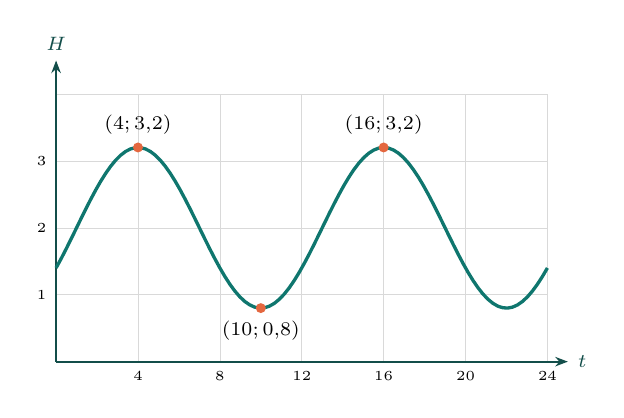
\begin{tikzpicture}[x=0.26cm,y=0.85cm]
\draw[gr] (0,0) grid[xstep=4,ystep=1] (24,4);
\draw[ax] (0,0)--(25,0) node[right,font=\scriptsize]{$t$};
\draw[ax] (0,0)--(0,4.5) node[above,font=\scriptsize]{$H$};
\draw[cur,domain=0:24,samples=100] plot (\x,{2+1.2*cos(30*(\x-4))});
\fill[coralx] (4,3.2) circle (1.8pt) (10,0.8) circle (1.8pt) (16,3.2) circle (1.8pt);
\node[font=\scriptsize,above] at (4,3.25) {$(4;3{,}2)$};
\node[font=\scriptsize,below] at (10,0.75) {$(10;0{,}8)$};
\node[font=\scriptsize,above] at (16,3.25) {$(16;3{,}2)$};
\foreach \t in {4,8,12,16,20,24}{\node[font=\tiny,below] at (\t,0) {\t};}
\foreach \h in {1,2,3}{\node[font=\tiny,left] at (0,\h) {\h};}
\end{tikzpicture}}}{\pil{$2$}{$3$}{$4$}{$5$}{$6$}}
\soal{\gbr{Gambar menunjukkan grafik fungsi $f$ dengan daerah asal $-2\le x\le4$. Tentukan apakah masing-masing pernyataan berikut Benar atau Salah.}{%
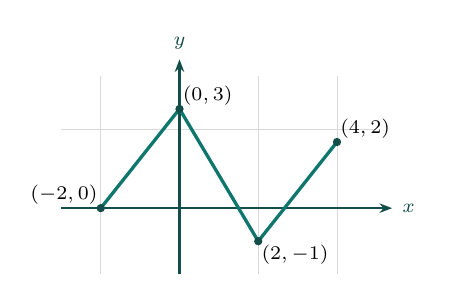
\begin{tikzpicture}[x=0.5cm,y=0.42cm]
\draw[gr] (-3,-2) grid (5,4);
\draw[ax] (-3,0)--(5.4,0) node[right,font=\scriptsize]{$x$};
\draw[ax] (0,-2)--(0,4.5) node[above,font=\scriptsize]{$y$};
\draw[cur] (-2,0)--(0,3)--(2,-1)--(4,2);
\fill[deepx] (-2,0) circle (1.5pt) (0,3) circle (1.5pt) (2,-1) circle (1.5pt) (4,2) circle (1.5pt);
\node[font=\scriptsize,above right,inner sep=1pt] at (0,3) {$(0,3)$};
\node[font=\scriptsize,below right,inner sep=1pt] at (2,-1) {$(2,-1)$};
\node[font=\scriptsize,above right,inner sep=1pt] at (4,2) {$(4,2)$};
\node[font=\scriptsize,above left,inner sep=1pt] at (-2,0) {$(-2,0)$};
\end{tikzpicture}}}{\begin{tabularx}{\linewidth}{@{}>{\raggedright\arraybackslash}X>{\centering\arraybackslash}p{1.3cm}>{\centering\arraybackslash}p{1.3cm}@{}}
\hline
\textbf{Pernyataan} & \textbf{Benar} & \textbf{Salah}\\ \hline
(1) Daerah hasil grafik $y=|f(x)|$ adalah $0\le y\le3$. & $\square$ & $\square$\\
(2) Daerah asal grafik $y=f(|x|)$ adalah $-2\le x\le4$. & $\square$ & $\square$\\
(3) Grafik $y=f(x-1)+2$ mencapai nilai minimum $1$ di $x=1$. & $\square$ & $\square$\\
(4) Persamaan $|f(x)|=1$ mempunyai tepat $4$ penyelesaian. & $\square$ & $\square$\\ \hline
\end{tabularx}}
\soal{\gbr{Lintasan sebuah roller coaster mini digambar pada bidang koordinat. Bagian pertama ($0\le x\le2$) berbentuk busur parabola $y=x(2-x)$. Bagian kedua ($2\le x\le4$) adalah bayangan bagian pertama oleh rotasi $180^\circ$ dengan pusat $(2,0)$. Pola sepanjang $4$ satuan ini kemudian diulang terus ke kanan dengan translasi $(4,0)$. Tinggi lintasan di $x=2026{,}5$ adalah \dots.}{%
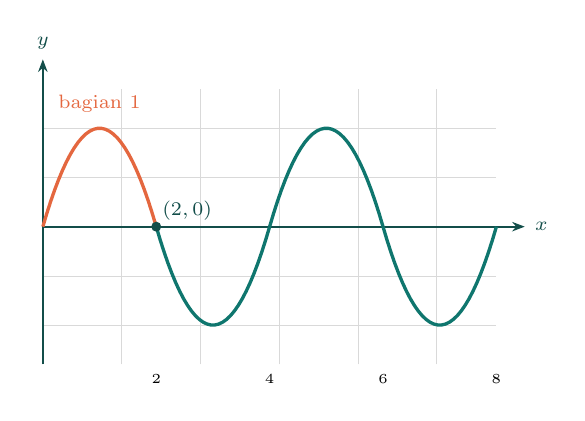
\begin{tikzpicture}[x=0.72cm,y=1.25cm]
\draw[gr] (0,-1.4) grid[ystep=0.5] (8,1.4);
\draw[ax] (0,0)--(8.5,0) node[right,font=\scriptsize]{$x$};
\draw[ax] (0,-1.4)--(0,1.7) node[above,font=\scriptsize]{$y$};
\draw[img,domain=0:2,samples=30] plot (\x,{\x*(2-\x)});
\draw[cur,domain=2:4,samples=30] plot (\x,{-(4-\x)*(\x-2)});
\draw[cur,domain=4:6,samples=30] plot (\x,{(\x-4)*(6-\x)});
\draw[cur,domain=6:8,samples=30] plot (\x,{-(8-\x)*(\x-6)});
\fill[deepx] (2,0) circle (1.8pt) node[above right,font=\scriptsize,inner sep=2pt]{$(2,0)$};
\foreach \t in {2,4,6,8}{\node[font=\tiny,below] at (\t,-1.4) {\t};}
\node[font=\scriptsize,coralx] at (1,1.25) {bagian 1};
\end{tikzpicture}}}{\pil{$-\frac34$}{$-\frac14$}{$\frac14$}{$\frac34$}{$-\frac32$}}
\soal{Parabola $y=x^2-4x+5$ ditranslasikan oleh $(p,q)$ sehingga bayangannya melalui titik asal $O(0,0)$. Berapakah nilai $p+q$?
\begin{enumerate}[label=(\arabic*),leftmargin=1.8em,itemsep=0pt,topsep=2pt]
\item $q=-2$.
\item Titik puncak bayangan terletak di kuadran III.
\end{enumerate}}{\begin{tabularx}{\linewidth}{@{}lX@{}}
\textbf{A.} & Pernyataan (1) SAJA cukup untuk menjawab pertanyaan, tetapi pernyataan (2) SAJA tidak cukup.\\
\textbf{B.} & Pernyataan (2) SAJA cukup untuk menjawab pertanyaan, tetapi pernyataan (1) SAJA tidak cukup.\\
\textbf{C.} & DUA pernyataan BERSAMA-SAMA cukup untuk menjawab pertanyaan, tetapi SATU pernyataan SAJA tidak cukup.\\
\textbf{D.} & Pernyataan (1) SAJA cukup dan pernyataan (2) SAJA cukup untuk menjawab pertanyaan.\\
\textbf{E.} & Pernyataan (1) dan pernyataan (2) tidak cukup untuk menjawab pertanyaan.
\end{tabularx}}

% =====================================================================
\newpage\bagian{B. Isian Singkat}{5 soal $\times$ 4 poin = 20 poin. Tuliskan hanya jawaban akhir.}

\tingkat{Tingkat Sedang}{soal 1 dan 2}
\soal{\gbr{Pada gambar, parabola $Q$ (garis tebal) diperoleh dari parabola $P:\ y=(x-2)^2-1$ (putus-putus) melalui pencerminan terhadap sumbu-$x$ yang dilanjutkan translasi $(a,b)$. Nilai $a+b$ adalah \dots.}{%
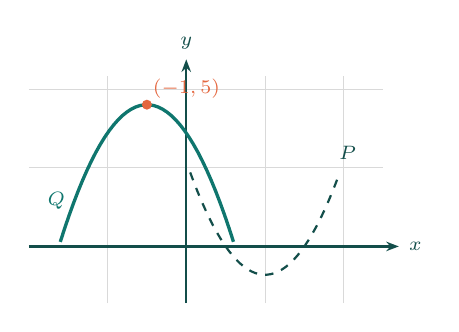
\begin{tikzpicture}[x=0.5cm,y=0.36cm]
\draw[gr] (-4,-2) grid (5,6);
\draw[ax] (-4,0)--(5.4,0) node[right,font=\scriptsize]{$x$};
\draw[ax] (0,-2)--(0,6.6) node[above,font=\scriptsize]{$y$};
\draw[orig,domain=0.1:3.9,samples=40] plot (\x,{(\x-2)^2-1});
\draw[cur,domain=-3.2:1.2,samples=40] plot (\x,{-(\x+1)^2+5});
\fill[coralx] (-1,5) circle (1.8pt) node[above right,font=\scriptsize,inner sep=2pt]{$(-1,5)$};
\node[font=\scriptsize,deepx] at (4.1,3.3) {$P$};
\node[font=\scriptsize,tealx] at (-3.3,1.6) {$Q$};
\end{tikzpicture}}}{\jwb}
\soal{Parabola $y=x^2-4x+3$ didilatasikan dengan pusat $O(0,0)$ dan faktor skala $-2$. Jika titik $(2,t)$ terletak pada parabola bayangan, nilai $t$ adalah \dots.}{\jwb}

\tingkat{Tingkat Sulit}{soal 3 sampai 5}
\soal{\gbr{Segitiga dengan titik sudut $O(0,0)$, $A(2,0)$, dan $B(0,3)$ (daerah arsiran gelap) ditransformasikan oleh matriks $M=\begin{pmatrix}2&-1\\1&3\end{pmatrix}$ menjadi segitiga bayangan (putus-putus). Luas segitiga bayangan adalah \dots\ satuan luas.}{%
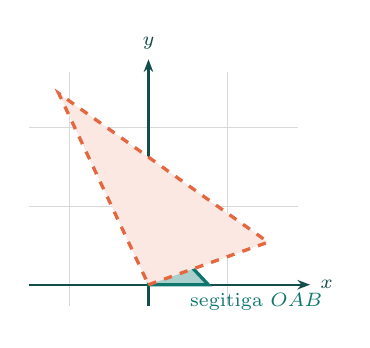
\begin{tikzpicture}[x=0.38cm,y=0.27cm]
\draw[gr] (-4,-1) grid (5,10);
\draw[ax] (-4,0)--(5.4,0) node[right,font=\scriptsize]{$x$};
\draw[ax] (0,-1)--(0,10.6) node[above,font=\scriptsize]{$y$};
\fill[tealx!35] (0,0)--(2,0)--(0,3)--cycle;
\draw[cur] (0,0)--(2,0)--(0,3)--cycle;
\fill[coralx!15] (0,0)--(4,2)--(-3,9)--cycle;
\draw[img,dashed] (0,0)--(4,2)--(-3,9)--cycle;
\node[font=\scriptsize,tealx] at (3.6,-0.8) {segitiga $OAB$};
\end{tikzpicture}}}{\jwb}
\soal{\gbr{Parabola $y=x^2$ dicerminkan terhadap garis $y=x+2$ sehingga menghasilkan kurva $\Gamma$ (garis tebal pada gambar). Jarak antara dua titik potong kurva $\Gamma$ dengan sumbu-$y$ adalah \dots.}{%
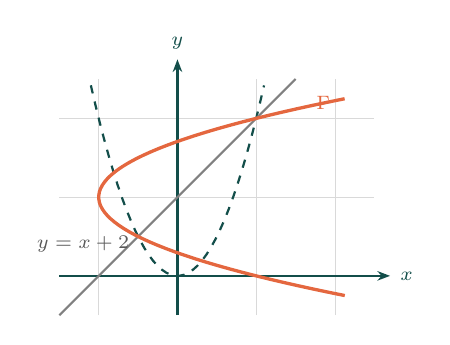
\begin{tikzpicture}[x=0.5cm,y=0.5cm]
\draw[gr] (-3,-1) grid (5,5);
\draw[ax] (-3,0)--(5.4,0) node[right,font=\scriptsize]{$x$};
\draw[ax] (0,-1)--(0,5.5) node[above,font=\scriptsize]{$y$};
\draw[orig,domain=-2.2:2.2,samples=40] plot (\x,{\x*\x});
\draw[gray,thick] (-3,-1)--(3,5);
\draw[img,domain=-0.5:4.5,samples=60] plot ({(\x-2)^2-2},{\x});
\node[font=\scriptsize,gray!70!black] at (-2.4,0.8) {$y=x+2$};
\node[font=\scriptsize,coralx] at (3.7,4.4) {$\Gamma$};
\end{tikzpicture}}}{\jwb}
\soal{Titik $P(3,2)$ dicerminkan secara berurutan terhadap garis $x=1$, kemudian garis $x=4$, kemudian garis $x=1$ lagi, kemudian garis $x=4$ lagi, dan seterusnya bergantian sehingga seluruhnya dilakukan $2027$ kali pencerminan. Jika koordinat titik akhir adalah $(a,b)$, nilai $a+b$ adalah \dots.}{\jwb}

% =====================================================================
\Needspace{16\baselineskip}
\bagian{C. Uraian (Essay)}{5 soal $\times$ 8 poin = 40 poin. Tuliskan langkah penyelesaian dengan lengkap.}

\tingkat{Tingkat Sedang}{soal 1 dan 2}
\soal{\gbr{Gambar menunjukkan grafik $f(x)=x^2$ (putus-putus) dan grafik $g$ berupa parabola dengan titik puncak $(3,5)$ yang melalui titik $(4,3)$. Grafik $g$ diperoleh dari grafik $f$ melalui peregangan vertikal, pencerminan, dan translasi.\par\smallskip
(a) Tulis $g(x)$ dalam bentuk $a\,f(x-h)+k$, lalu tentukan $a$, $h$, dan $k$.\par
(b) Jelaskan urutan transformasi dari $f$ ke $g$, dan tunjukkan bahwa jika translasi dikerjakan lebih dulu, hasilnya berbeda.\par
(c) Tentukan titik potong $g$ dengan sumbu-$y$ dan sumbu-$x$.\par
(d) Garis $y=-3$ memotong $g$ di dua titik. Tentukan panjang ruas garis yang terpotong, lalu tentukan persamaan bayangan $g$ oleh pencerminan terhadap garis $y=1$.}{%
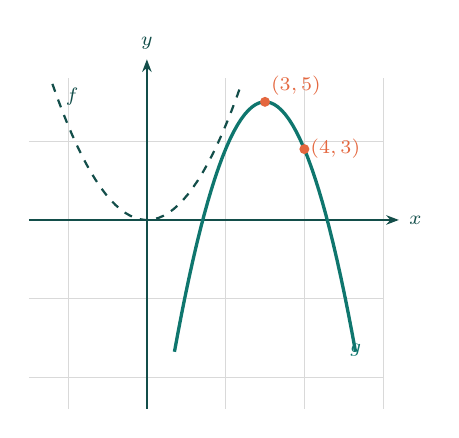
\begin{tikzpicture}[x=0.5cm,y=0.3cm]
\draw[gr] (-3,-8) grid (6,6);
\draw[ax] (-3,0)--(6.4,0) node[right,font=\scriptsize]{$x$};
\draw[ax] (0,-8)--(0,6.8) node[above,font=\scriptsize]{$y$};
\draw[orig,domain=-2.4:2.4,samples=40] plot (\x,{\x*\x});
\draw[cur,domain=0.7:5.3,samples=50] plot (\x,{-2*(\x-3)^2+5});
\fill[coralx] (3,5) circle (1.8pt) node[above right,font=\scriptsize,inner sep=2pt]{$(3,5)$};
\fill[coralx] (4,3) circle (1.8pt) node[right,font=\scriptsize,inner sep=2pt]{$(4,3)$};
\node[font=\scriptsize,deepx] at (-1.9,5.2) {$f$};
\node[font=\scriptsize,tealx] at (5.3,-5.5) {$g$};
\end{tikzpicture}}}{\poin{8}}
\soal{\gbr{Segitiga $ABC$ dengan $A(1,1)$, $B(5,1)$, dan $C(5,4)$ ditransformasikan secara berurutan oleh: $T_1$ rotasi $90^\circ$ dengan pusat $O$, $T_2$ dilatasi $[O,2]$, dan $T_3$ translasi $(4,-1)$. Bayangan akhirnya adalah segitiga $A''B''C''$.\par\smallskip
(a) Tentukan koordinat bayangan setiap titik setelah $T_1$, setelah $T_2$, dan setelah $T_3$.\par
(b) Tentukan matriks $M$ untuk komposisi $T_1$ dilanjutkan $T_2$, lalu tuliskan rumus pemetaan $(x,y)\to(x'',y'')$ untuk ketiga transformasi, dan periksa dengan titik $C$.\par
(c) Hitung perbandingan keliling dan perbandingan luas segitiga $A''B''C''$ terhadap $ABC$, lalu jelaskan hasilnya.\par
(d) Tentukan persamaan bayangan garis $AC$.}{%
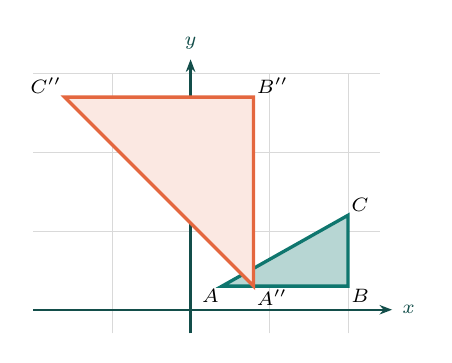
\begin{tikzpicture}[x=0.4cm,y=0.3cm]
\draw[gr] (-5,-1) grid (6,10);
\draw[ax] (-5,0)--(6.4,0) node[right,font=\scriptsize]{$x$};
\draw[ax] (0,-1)--(0,10.6) node[above,font=\scriptsize]{$y$};
\fill[tealx!30] (1,1)--(5,1)--(5,4)--cycle;
\draw[cur] (1,1)--(5,1)--(5,4)--cycle;
\fill[coralx!15] (2,1)--(2,9)--(-4,9)--cycle;
\draw[img] (2,1)--(2,9)--(-4,9)--cycle;
\node[font=\scriptsize,below left,inner sep=1pt] at (1,1) {$A$};
\node[font=\scriptsize,below right,inner sep=1pt] at (5,1) {$B$};
\node[font=\scriptsize,above right,inner sep=1pt] at (5,4) {$C$};
\node[font=\scriptsize,below right,inner sep=1pt] at (2,1) {$A''$};
\node[font=\scriptsize,above right,inner sep=1pt] at (2,9) {$B''$};
\node[font=\scriptsize,above left,inner sep=1pt] at (-4,9) {$C''$};
\end{tikzpicture}}}{\poin{8}}

\tingkat{Tingkat Sulit}{soal 3 dan 4}
\soal{\gbr{Diketahui $f(x)=x^2-4x-5$ dengan grafik seperti pada gambar. Misalkan $g(x)=|f(x)|$ dan $h(x)=f(|x|)$.\par\smallskip
(a) Tentukan titik potong grafik $f$ dengan sumbu-koordinat dan titik puncaknya. Jelaskan cara memperoleh grafik $g$ dan $h$ dari grafik $f$, lalu sebutkan titik ekstrem lokal masing-masing.\par
(b) Tentukan semua nilai $k$ sehingga $g(x)=k$ memiliki tepat $3$ penyelesaian, lalu tentukan penyelesaiannya.\par
(c) Tentukan semua nilai $k$ sehingga $h(x)=k$ memiliki tepat $3$ penyelesaian, dan semua nilai $k$ sehingga $h(x)=k$ memiliki tepat $4$ penyelesaian.\par
(d) Tentukan semua nilai $k$ sehingga persamaan $|f(|x|)|=k$ memiliki tepat $6$ penyelesaian real.}{%
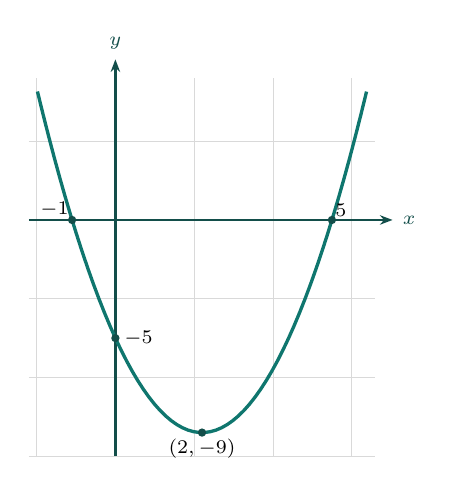
\begin{tikzpicture}[x=0.55cm,y=0.3cm]
\draw[gr] (-2,-10) grid (6,6);
\draw[ax] (-2,0)--(6.4,0) node[right,font=\scriptsize]{$x$};
\draw[ax] (0,-10)--(0,6.8) node[above,font=\scriptsize]{$y$};
\draw[cur,domain=-1.8:5.8,samples=60] plot (\x,{\x*\x-4*\x-5});
\fill[deepx] (-1,0) circle (1.5pt) (5,0) circle (1.5pt) (2,-9) circle (1.5pt) (0,-5) circle (1.5pt);
\node[font=\scriptsize,above left,inner sep=1pt] at (-1,0) {$-1$};
\node[font=\scriptsize,above right,inner sep=1pt] at (5,0) {$5$};
\node[font=\scriptsize,below,inner sep=2pt] at (2,-9) {$(2,-9)$};
\node[font=\scriptsize,right,inner sep=3pt] at (0,-5) {$-5$};
\end{tikzpicture}}}{\poin{8}}
\soal{\gbr{Diketahui $g(x)=\dfrac{2x+3}{x-2}$ dengan grafik seperti pada gambar (garis putus-putus tipis adalah asimtot dan garis $y=x$).\par\smallskip
(a) Tunjukkan bahwa $g(x)=2+\dfrac{7}{x-2}$, lalu jelaskan urutan transformasi dari grafik $y=\dfrac1x$ ke grafik $g$. Tentukan asimtot dan titik potong dengan sumbu-koordinat.\par
(b) Buktikan bahwa $g(2+t)+g(2-t)=4$ untuk setiap $t\ne0$, lalu tafsirkan secara geometris.\par
(c) Tunjukkan bahwa bayangan grafik $g$ oleh pencerminan terhadap garis $y=x$ adalah grafik $g$ itu sendiri, dan jelaskan hubungannya dengan letak titik $(2,2)$.\par
(d) Tentukan nilai $k$ sehingga garis $y=-x+k$ menyinggung grafik $g$. Jelaskan mengapa jumlah kedua nilai $k$ sama dengan $8$.}{%
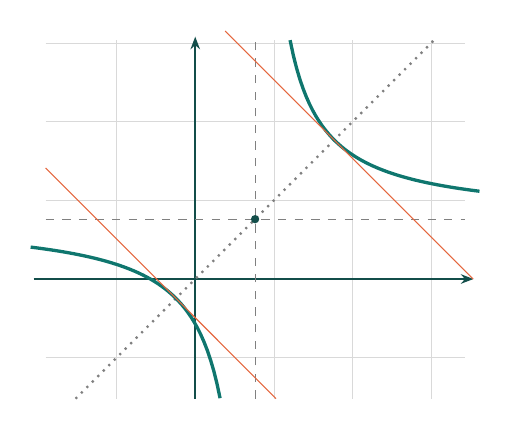
\begin{tikzpicture}[x=0.38cm,y=0.38cm]
\clip (-5.6,-4.2) rectangle (9.6,8.4);
\draw[gr] (-5,-4) grid (9,8);
\draw[ax] (-5.4,0)--(9.3,0) node[right,font=\scriptsize]{$x$};
\draw[ax] (0,-4)--(0,8.1) node[above,font=\scriptsize]{$y$};
\draw[gray,dashed] (2,-4)--(2,8) (-5,2)--(9,2);
\draw[gray,dotted,thick] (-4,-4)--(8,8);
\draw[cur,domain=3.17:9.5,samples=60] plot (\x,{2+7/(\x-2)});
\draw[cur,domain=-5.5:0.83,samples=60] plot (\x,{2+7/(\x-2)});
\draw[img,thin] (1,8.29)--(9.29,0) (-5,3.71)--(-1.29,0)--(2.7,-4);
\fill[deepx] (2,2) circle (1.5pt);
\end{tikzpicture}}}{\poin{8}}

\Needspace{22\baselineskip}\tingkat{Tingkat HOTS}{soal 5}
\soal{\gbr{Sebuah meja biliar berbentuk persegi panjang dengan sudut $(0,0)$, $(10,0)$, $(10,8)$, dan $(0,8)$ (satuan dm). Bola putih berada di $A(2,5)$ dan bola target di $B(6,2)$. Bola putih ditembakkan sehingga memantul lebih dulu di bantalan atas ($y=8$) di titik $P$, kemudian di bantalan kanan ($x=10$) di titik $Q$, lalu mengenai $B$. Pantulan mengikuti hukum: sudut datang sama dengan sudut pantul.\par\smallskip
(a) Tuliskan aturan pemetaan titik $(x,y)$ oleh pencerminan terhadap $x=10$ dan terhadap $y=8$.\par
(b) Tentukan koordinat $B^{*}$, yaitu bayangan $B$ oleh pencerminan terhadap $x=10$ dilanjutkan pencerminan terhadap $y=8$.\par
(c) Dengan meluruskan lintasan $A\to B^{*}$, tentukan koordinat $P$ dan $Q$, lalu periksa bahwa sudut datang sama dengan sudut pantul di $P$.\par
(d) Tentukan panjang seluruh lintasan, bandingkan dengan lintasan yang hanya memantul sekali di bantalan atas, dan jelaskan mengapa panjang lintasan dapat ditentukan tanpa mencari $P$ dan $Q$ lebih dulu.}{%
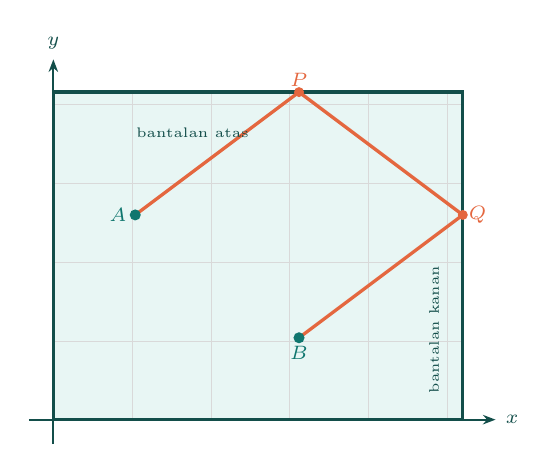
\begin{tikzpicture}[x=0.52cm,y=0.52cm]
\fill[softbg] (0,0) rectangle (10,8);
\draw[gr] (0,0) grid (10,8);
\draw[ax] (-0.6,0)--(10.8,0) node[right,font=\scriptsize]{$x$};
\draw[ax] (0,-0.6)--(0,8.8) node[above,font=\scriptsize]{$y$};
\draw[very thick,deepx] (0,0) rectangle (10,8);
\draw[img] (2,5)--(6,8)--(10,5)--(6,2);
\fill[tealx] (2,5) circle (2pt) node[left,font=\scriptsize,inner sep=3pt]{$A$};
\fill[tealx] (6,2) circle (2pt) node[below,font=\scriptsize,inner sep=3pt]{$B$};
\fill[coralx] (6,8) circle (1.8pt) node[above,font=\scriptsize,inner sep=2pt]{$P$};
\fill[coralx] (10,5) circle (1.8pt) node[right,font=\scriptsize,inner sep=2pt]{$Q$};
\node[font=\tiny,deepx] at (3.4,7.0) {bantalan atas};
\node[font=\tiny,deepx,rotate=90] at (9.3,2.2) {bantalan kanan};
\end{tikzpicture}}}{\poin{8}}

% =====================================================================
\newpage
\bagian{Kunci Jawaban dan Pembahasan Singkat}{Untuk guru dan pembahasan mandiri}
\par\vspace{0.6em}{\bfseries\color{tealx}Kunci Pilihan Ganda}\par\vspace{0.3em}
\small
\begin{tabularx}{\linewidth}{@{}*{10}{>{\centering\arraybackslash}X}@{}}\hline \textbf{1} & \textbf{2} & \textbf{3} & \textbf{4} & \textbf{5} & \textbf{6} & \textbf{7} & \textbf{8} & \textbf{9} & \textbf{10}\\ \hline B & C & E & A & D & B & A & C & E & D\\ \hline\end{tabularx}\\[6pt]
\begin{tabularx}{\linewidth}{@{}*{10}{>{\centering\arraybackslash}X}@{}}\hline \textbf{11} & \textbf{12} & \textbf{13} & \textbf{14} & \textbf{15} & \textbf{16} & \textbf{17} & \textbf{18} & \textbf{19} & \textbf{20}\\ \hline C & B & A & E & D & B & C & {\scriptsize B,S,S,B} & A & C\\ \hline\end{tabularx}
\par\vspace{0.8em}{\bfseries\color{tealx}\normalsize Pembahasan Pilihan Ganda}\par\vspace{0.2em}
\small\begin{enumerate}[leftmargin=2em,itemsep=2pt,topsep=2pt]
\item[\textbf{1.}] \textbf{(B)} $g(x)=f(x+3)-1$ berarti grafik $f$ digeser $3$ satuan ke \emph{kiri} dan $1$ satuan ke bawah, yaitu translasi $(-3,-1)$. Titik minimum $f$ adalah $(1,-2)$, bayangannya $(1-3,-2-1)=(-2,-3)$. (Jebakan A dan D: menggeser ke kanan.)
\item[\textbf{2.}] \textbf{(C)} Pencerminan terhadap $x=1$: $(x,y)\to(2-x,y)$. Substitusi $x\to2-x$: $2(2-x)-y+4=0\Rightarrow2x+y-8=0$. Cek: titik $(0,4)$ pada garis semula menjadi $(2,4)$ dan $4+4-8=0$. (Jebakan A: memakai pencerminan terhadap sumbu-$y$.)
\item[\textbf{3.}] \textbf{(E)} Pada $y=\frac12f(3x)$, nilai maksimum $f$ muncul ketika $3x=2$, yaitu $x=\frac23$ (mampat horizontal $\frac13$), dan tingginya menjadi $\frac12\cdot6=3$. Jadi titiknya $\left(\frac23,3\right)$.
\item[\textbf{4.}] \textbf{(A)} Rotasi $90^\circ$: $(x,y)\to(-y,x)$, sehingga $x'=-y$ dan $y'=x$. Dari $y=2x+1$: $-x'=2y'+1\Rightarrow y'=-\frac12x'-\frac12$. Cek: $(0,1)\to(-1,0)$ dan $-\frac12(-1)-\frac12=0$. (Gradien hasil rotasi $90^\circ$ adalah $-\frac1m$.)
\item[\textbf{5.}] \textbf{(D)} Titik puncak $y=x^2-2x-3$ adalah $(1,-4)$. Pada $y=|f(x)|$, bagian di bawah sumbu-$x$ dicerminkan ke atas, sehingga $(1,-4)$ menjadi maksimum lokal $(1,4)$.
\item[\textbf{6.}] \textbf{(B)} Pencerminan terhadap $y=1$: $y=2-f(x)=-x^2+6x-5$. Translasi $(-2,3)$: ganti $x\to x+2$ dan $y\to y-3$: $y-3=-(x+2)^2+6(x+2)-5\Rightarrow y=-x^2+2x+6$. (Jebakan A: translasi dikerjakan lebih dulu, lalu dicerminkan.)
\item[\textbf{7.}] \textbf{(A)} $T_1$: $(x,y)\to(-y,-x)$. $T_2$: $(u,v)\to(-v,u)$. Komposisi: $(x,y)\to(-y,-x)\to(x,-y)$, yaitu pencerminan terhadap sumbu-$x$. Maka $(a,-b)=(-3,5)$, sehingga $a=-3$, $b=-5$, dan $a+b=-8$. (Jebakan B: urutan dibalik.)
\item[\textbf{8.}] \textbf{(C)} Puncak $y=x^2-4x+3$ adalah $(2,-1)$. Pada grafik mutlak, titik ini menjadi maksimum lokal $(2,1)$. Garis $y=m$ memotong di tepat tiga titik saat melalui maksimum lokal tersebut: $m=1$. Penyelesaiannya $x=2$ dan $x=2\pm\sqrt2$.
\item[\textbf{9.}] \textbf{(E)} Dilatasi $[P(1,2),2]$: $(x,y)\to(1+2(x-1),\,2+2(y-2))=(2x-1,2y-2)$. Maka $x=\frac{x'+1}2$ dan $y=\frac{y'+2}2$. Substitusi ke $y=x^2$: $\frac{y'+2}2=\frac{(x'+1)^2}4\Rightarrow y'=\frac12x'^2+x'-\frac32$. (Jebakan B: pusat dianggap $O$.)
\item[\textbf{10.}] \textbf{(D)} Dari $g(x)=2f(x+1)-3$ diperoleh $f(x+1)=\frac{g(x)+3}2$. $f(0)$: $x=-1$, $g=-3$, sehingga $f(0)=0$. $f(2)$: $x=1$, $g=3$, sehingga $f(2)=3$. $f(4)$: $x=3$, $g=-1$, sehingga $f(4)=1$. Jumlah $=4$.
\item[\textbf{11.}] \textbf{(C)} $g(x)=-2f(-(x-3))+4$. Titik $f(t)$ dengan $t=-1$ memberi $x=3-t=4$. Karena $f(t)\ge5$ untuk semua $t$, maka $-2f\le-10$ dan $g\le-10+4=-6$. Jadi maksimum global di $(4,-6)$. (Jebakan A: salah arah geser; B dan D: lupa pencerminan sumbu-$x$ membalik minimum menjadi maksimum.)
\item[\textbf{12.}] \textbf{(B)} Rotasi $90^\circ$: $(x,y)\to(-y,x)$. Titik $(x_0,\log_2x_0)$ menjadi $(X,Y)=(-\log_2x_0,x_0)$, sehingga $X=-\log_2Y$ dan $Y=2^{-X}$. Translasi $(1,-3)$: $y=2^{-(x-1)}-3=2^{1-x}-3$. Titik potong sumbu-$x$: $2^{1-x}=3\Rightarrow1-x=\log_23\Rightarrow x=1-\log_23$.
\item[\textbf{13.}] \textbf{(A)} Rotasi $180^\circ$ pusat $(a,b)$: $(x,y)\to(2a-x,2b-y)$, jadi bayangan $y=20-(6-x)^2=-x^2+12x-16$. Perpotongan: $x^2=-x^2+12x-16\Rightarrow x^2-6x+8=0\Rightarrow x=2$ atau $4$. Titiknya $(2,4)$ dan $(4,16)$ (titik tengahnya tepat $C(3,10)$). Jarak $=\sqrt{2^2+12^2}=\sqrt{148}=2\sqrt{37}$.
\item[\textbf{14.}] \textbf{(E)} Kurva $A$: $y=|x|-2$. Kurva $B$: $-|x|\to-2|x|\to y=4-2|x|$. Perpotongan: $|x|-2=4-2|x|\Rightarrow|x|=2$, titik $(\pm2,0)$. Daerah berbentuk layang-layang dengan titik sudut $(0,-2)$, $(2,0)$, $(0,4)$, $(-2,0)$. Diagonalnya $4$ dan $6$, sehingga luas $=\frac12\cdot4\cdot6=12$.
\item[\textbf{15.}] \textbf{(D)} Translasi $(1,-2)$: $y+2=(x-1)^2-2(x-1)\Rightarrow y=x^2-4x+1$. Pencerminan sumbu-$x$: $P:\ y=-x^2+4x-1$. Menyinggung $y=3x+k$: $-x^2+4x-1=3x+k\Rightarrow x^2-x+(1+k)=0$. Diskriminan nol: $1-4(1+k)=0\Rightarrow k=-\frac34$.
\item[\textbf{16.}] \textbf{(B)} Langkah 1 dan 2 benar. Pada langkah 3: $\frac{y'}2=\frac{x'^2}4-x'$; kedua ruas dikalikan $2$ memberi $y'=\frac12x'^2-2x'$ (suku $-x'$ juga harus dikali $2$), sedangkan Rani menulis $-x'$. Langkah 4 dan 5 konsisten dengan kesalahan itu. Yang benar: translasi $(1,-1)$ memberi $y+1=\frac12(x-1)^2-2(x-1)\Rightarrow y=\frac12x^2-3x+\frac32$.
\item[\textbf{17.}] \textbf{(C)} Dari grafik: maksimum $3{,}2$ dan minimum $0{,}8$, sehingga amplitudo $\frac{3{,}2-0{,}8}2=1{,}2$ dan garis tengah $2$. Dua maksimum berurutan di $t=4$ dan $t=16$, jadi periode $12$ dan $b=\frac{2\pi}{12}=\frac\pi6$. Model: $H(t)=2+1{,}2\cos\frac\pi6(t-4)$. Syarat $H\ge2{,}6$: $\cos\frac\pi6(t-4)\ge\frac12\Rightarrow\left|\frac\pi6(t-4)\right|\le\frac\pi3\Rightarrow|t-4|\le2$, yaitu $2\le t\le6$. Lamanya $4$ jam.
\item[\textbf{18.}] \textbf{(B, S, S, B)} Titik ekstrem $f$: maksimum $3$ di $x=0$, minimum $-1$ di $x=2$. (1) \emph{Benar}: pada $|f|$, nilai $-1$ menjadi $1$, sehingga daerah hasil $0\le y\le3$ (nilai $0$ dicapai di pembuat nol $f$). (2) \emph{Salah}: $f(|x|)$ terdefinisi jika $-2\le|x|\le4$, yaitu $|x|\le4$, sehingga daerah asalnya $-4\le x\le4$. (3) \emph{Salah}: minimum $f$ di $(2,-1)$ bergeser ke $(3,1)$, jadi minimum $1$ terjadi di $x=3$, bukan $x=1$. (4) \emph{Benar}: $f(x)=1$ di $x=-\frac43$, $1$, dan $\frac{10}3$ (tiga penyelesaian); $f(x)=-1$ hanya di $x=2$. Total $4$ penyelesaian.
\item[\textbf{19.}] \textbf{(A)} Bagian kedua: rotasi $180^\circ$ pusat $(2,0)$ memetakan $(x,y)\to(4-x,-y)$, sehingga untuk $2\le x\le4$ berlaku $y=-(4-x)(x-2)$. Pola berulang setiap $4$ satuan. $2026{,}5=4\cdot506+2{,}5$, sehingga tinggi di $x=2026{,}5$ sama dengan tinggi di $x=2{,}5$: $y=-(4-2{,}5)(2{,}5-2)=-(1{,}5)(0{,}5)=-\frac34$.
\item[\textbf{20.}] \textbf{(C)} Bayangan: $y=(x-p)^2-4(x-p)+5+q$. Melalui $O$: $p^2+4p+5+q=0$, sehingga $q=-(p^2+4p+5)$ (satu persamaan dua variabel). Titik puncak semula $(2,1)$, bayangannya $(2+p,1+q)$. Pernyataan (1): $q=-2\Rightarrow p^2+4p+3=0\Rightarrow p=-1$ atau $p=-3$, sehingga $p+q=-3$ atau $-5$; tidak cukup. Pernyataan (2): kuadran III berarti $p<-2$ dan $q<-1$, ada tak hingga pasangan; tidak cukup. Bersama-sama: $q=-2$ dan $p<-2$ memberi $p=-3$, sehingga $p+q=-5$. Cukup.
\end{enumerate}
\par\Needspace{6\baselineskip}\vspace{0.6em}{\bfseries\color{tealx}\normalsize Pembahasan Isian Singkat}\par\vspace{0.2em}
\small\begin{enumerate}[leftmargin=2em,itemsep=2pt,topsep=2pt]
\item[\textbf{1.}] \textbf{Jawaban: $1$.} Puncak $P$ adalah $(2,-1)$. Pencerminan terhadap sumbu-$x$ memberi $(2,1)$. Puncak $Q$ pada gambar adalah $(-1,5)$, sehingga $(2+a,1+b)=(-1,5)\Rightarrow a=-3$ dan $b=4$. Jadi $a+b=1$. (Konsisten: $Q$ terbuka ke bawah.)
\item[\textbf{2.}] \textbf{Jawaban: $-16$.} Dilatasi $[O,k]$: $y=k\,f\!\left(\frac xk\right)$ dengan $k=-2$. Di $x=2$: $t=-2f(-1)=-2(1+4+3)=-16$. (Titik asal $(-1,8)$ dipetakan ke $(2,-16)$.)
\item[\textbf{3.}] \textbf{Jawaban: $21$.} Bayangan titik: $O\to(0,0)$, $A(2,0)\to(4,2)$, $B(0,3)\to(-3,9)$. Luas $=\frac12|4\cdot9-(-3)\cdot2|=\frac12\cdot42=21$. Sebagai pemeriksaan, $\det M=2\cdot3-(-1)(1)=7$ dan luas awal $3$, sehingga $7\times3=21$.
\item[\textbf{4.}] \textbf{Jawaban: $2\sqrt2$.} Pencerminan terhadap $y=x+2$: $(x,y)\to(y-2,x+2)$. Maka $X=y-2$ dan $Y=x+2$, sehingga $x=Y-2$ dan $y=X+2$. Dari $y=x^2$: $X=(Y-2)^2-2$. Di sumbu-$y$ ($X=0$): $(Y-2)^2=2\Rightarrow Y=2\pm\sqrt2$. Jarak $=2\sqrt2$.
\item[\textbf{5.}] \textbf{Jawaban: $-6077$.} Dua pencerminan berurutan terhadap garis sejajar $x=1$ lalu $x=4$ sama dengan translasi sejauh $2(4-1)=6$ ke kanan: $3\to-1\to9$. Setelah $2026=2\cdot1013$ pencerminan, absis $=3+6\cdot1013=6081$ dan ordinat tetap $2$. Pencerminan ke-$2027$ terhadap $x=1$: $2\cdot1-6081=-6079$. Titik akhir $(-6079,2)$ dan $a+b=-6077$.
\end{enumerate}
\par\Needspace{8\baselineskip}\vspace{0.6em}{\bfseries\color{tealx}\normalsize Pembahasan dan Pedoman Penskoran Uraian}\par\vspace{0.2em}
\small\begin{enumerate}[leftmargin=2em,itemsep=3pt,topsep=2pt]
\item[\textbf{1.}] (a) $g(x)=-2(x-3)^2+5=-2f(x-3)+5$, sehingga $a=-2$, $h=3$, $k=5$ (titik $(4,3)$: $-2+5=3$, cocok). (b) Urutan: regang vertikal faktor $2$: $y=2x^2$; cermin terhadap sumbu-$x$: $y=-2x^2$; translasi $(3,5)$: $y=-2(x-3)^2+5$. Jika translasi lebih dulu: $y=(x-3)^2+5$, lalu regang dan cermin menghasilkan $y=-2(x-3)^2-10$, titik puncaknya $(3,-10)$, berbeda dari $(3,5)$. (c) Sumbu-$y$: $g(0)=-18+5=-13$, titik $(0,-13)$. Sumbu-$x$: $(x-3)^2=\frac52\Rightarrow x=3\pm\frac{\sqrt{10}}2$. (d) $-2(x-3)^2+5=-3\Rightarrow(x-3)^2=4\Rightarrow x=1$ atau $5$, panjang ruas $4$. Pencerminan terhadap $y=1$: $y=2-g(x)=2(x-3)^2-3$. \\ \textit{Penskoran: (a) 2 poin; (b) 2 poin; (c) 2 poin; (d) 2 poin.}
\item[\textbf{2.}] (a) $T_1:(x,y)\to(-y,x)$: $A'(-1,1)$, $B'(-1,5)$, $C'(-4,5)$. $T_2$: $A''(-2,2)$, $B''(-2,10)$, $C''(-8,10)$ (setelah dilatasi). $T_3$ (translasi $(4,-1)$): $(2,1)$, $(2,9)$, $(-4,9)$. (b) $M=\begin{pmatrix}2&0\\0&2\end{pmatrix}\begin{pmatrix}0&-1\\1&0\end{pmatrix}=\begin{pmatrix}0&-2\\2&0\end{pmatrix}$. Pemetaan total: $(x,y)\to(-2y+4,\;2x-1)$. Cek $C(5,4)$: $(-8+4,10-1)=(-4,9)$. (c) $AB=4$, $BC=3$, $AC=5$ (keliling $12$); $A''B''=8$, $B''C''=6$, $A''C''=10$ (keliling $24$). Rasio keliling $2$. Luas $ABC=6$ dan $A''B''C''=\frac12\cdot8\cdot6=24$, rasio luas $4$. Rotasi dan translasi mempertahankan ukuran; dilatasi faktor $2$ melipatkan panjang $2$ kali dan luas $2^2=4$ kali ($|\det M|=4$). (d) Garis $AC$: $3x-4y+1=0$. Dari pemetaan: $x=\frac{y''+1}2$ dan $y=\frac{4-x''}2$. Substitusi: $\frac{3(y''+1)}2-2(4-x'')+1=0\Rightarrow4x+3y-11=0$. Cek: $A''(2,1)$ dan $C''(-4,9)$ memenuhi. \\ \textit{Penskoran: (a) 2 poin; (b) 2 poin; (c) 2 poin; (d) 2 poin.}
\item[\textbf{3.}] (a) $f$: sumbu-$x$ di $-1$ dan $5$, sumbu-$y$ di $-5$, puncak $(2,-9)$. $g=|f|$: bagian di bawah sumbu-$x$ dicerminkan ke atas, ekstrem lokal: maksimum $(2,9)$, minimum $(-1,0)$ dan $(5,0)$. $h=f(|x|)$: bagian $x\ge0$ dipertahankan, lalu dicerminkan terhadap sumbu-$y$ sebagai pengganti bagian kiri; ekstrem lokal: minimum $(\pm2,-9)$ dan maksimum lokal $(0,-5)$. (b) $|f(x)|=k$ tepat $3$ penyelesaian saat $k=9$ (garis melalui maksimum lokal). $x^2-4x-5=9\Rightarrow x=2\pm3\sqrt2$, dan $-f(x)=9\Rightarrow x=2$. (c) $f(|x|)=k$: tepat $3$ penyelesaian jika $k=-5$ ($x=0$ dan $x=\pm4$); tepat $4$ penyelesaian jika $-9<k<-5$. (d) Untuk $x\ge0$, $|h|$ naik dari $5$ (di $x=0$) ke $9$ (di $x=2$), turun ke $0$ (di $x=5$), lalu naik tak terbatas; grafik simetris terhadap sumbu-$y$. Untuk $5<k<9$ setiap sisi ($x>0$) memberi $3$ penyelesaian, total $6$. Untuk $k=5$ ada $5$ penyelesaian, $k=9$ ada $4$, $0<k<5$ ada $4$, $k>9$ ada $2$. Jadi $5<k<9$. \\ \textit{Penskoran: (a) 2 poin; (b) 2 poin; (c) 2 poin; (d) 2 poin.}
\item[\textbf{4.}] (a) $\frac{2x+3}{x-2}=\frac{2(x-2)+7}{x-2}=2+\frac7{x-2}$. Dari $y=\frac1x$: regang vertikal faktor $7$ ($y=\frac7x$), lalu translasi $(2,2)$. Asimtot $x=2$ dan $y=2$. Sumbu-$x$: $\left(-\frac32,0\right)$; sumbu-$y$: $\left(0,-\frac32\right)$. (b) $g(2+t)=2+\frac7t$ dan $g(2-t)=2-\frac7t$; jumlahnya $4$. Artinya titik $(2+t,\,g(2+t))$ dan $(2-t,\,g(2-t))$ berjarak sama dari $(2,2)$ pada arah berlawanan; grafik simetris titik terhadap $(2,2)$ (pusat hiperbola). (c) Pencerminan terhadap $y=x$ menukar $x$ dan $y$: $x=\frac{2y+3}{y-2}\Rightarrow xy-2x=2y+3\Rightarrow y(x-2)=2x+3\Rightarrow y=\frac{2x+3}{x-2}$, sama dengan $g$. Sebab: pusat $(2,2)$ terletak pada $y=x$ dan kedua asimtot ($x=2$ dan $y=2$) saling dicerminkan oleh $y=x$. (d) $2+\frac7{x-2}=-x+k\Rightarrow2x+3=(-x+k)(x-2)\Rightarrow x^2-kx+2k+3=0$. Menyinggung: $D=k^2-4(2k+3)=0\Rightarrow k^2-8k-12=0\Rightarrow k=4\pm2\sqrt7$. Jumlahnya $8$ (Vieta). Secara geometri, kedua garis tegak lurus cermin $y=x$ dan saling bayangan terhadap titik $(2,2)$ (simetri titik), sehingga $k_1+k_2=2(2+2)=8$. \\ \textit{Penskoran: (a) 2 poin; (b) 2 poin; (c) 2 poin; (d) 2 poin.}
\item[\textbf{5.}] (a) Terhadap $x=10$: $(x,y)\to(20-x,y)$. Terhadap $y=8$: $(x,y)\to(x,16-y)$. (b) $B(6,2)\to(14,2)\to(14,14)$, sehingga $B^{*}=(14,14)$. (c) Gradien $AB^{*}=\frac{14-5}{14-2}=\frac34$; garis $y-5=\frac34(x-2)$. Memotong $y=8$ di $x=6$, jadi $P(6,8)$. Pada $x=10$ garis (lintasan terlipat) berada di $y=5+\frac34\cdot8=11$; dilipat terhadap $y=8$ menjadi $16-11=5$, jadi $Q(10,5)$. Pemeriksaan: gradien $AP=\frac34$, $PQ=-\frac34$, $QB=\frac34$. Di $P$ gradien berubah tanda dengan besar sama sehingga sudut datang sama dengan sudut pantul; $QB$ juga konsisten. (d) Panjang lintasan $=AP+PQ+QB=5+5+5=15$ dm, sama dengan $AB^{*}=\sqrt{12^2+9^2}=15$ karena pencerminan mempertahankan jarak, sehingga setiap segmen lintasan "diluruskan" menjadi bagian dari garis lurus $AB^{*}$. Lintasan satu pantulan lewat bantalan atas: $B'=(6,14)$, panjang $\sqrt{4^2+9^2}=\sqrt{97}\approx9{,}8<15$. Jadi lintasan dua pantulan lebih panjang. \\ \textit{Penskoran: (a) 1 poin; (b) 2 poin; (c) 3 poin (P 1, Q 1, pemeriksaan 1); (d) 2 poin.}
\end{enumerate}
\end{document}
